69. Один литр --- это кубический дециметр. На уроке труда Вася сделал стальную заготовку для ванны с прямоугольным основанием, изображённую на схеме (пунктирные линии обозначают места сгиба). Сторона одной клеточки равна 1 дециметру. Сварив края ванны, Вася обнаружил, что она вышла кривая. Какое наибольшее количество литров воды войдёт в ванну?
\begin{center}
\begin{figure}[ht!]
\center{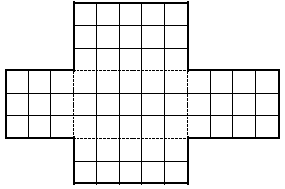
\includegraphics[scale=0.35]{13.png}}
\end{figure}
\end{center}
